\chapter{Simulation}\label{chap:Simulation}

\section{CFD}\label{sec:sim_cfd}

\begin{figure}[H]
    \centering
    \begin{subfigure}[t]{0.7\textwidth}
        \centering
        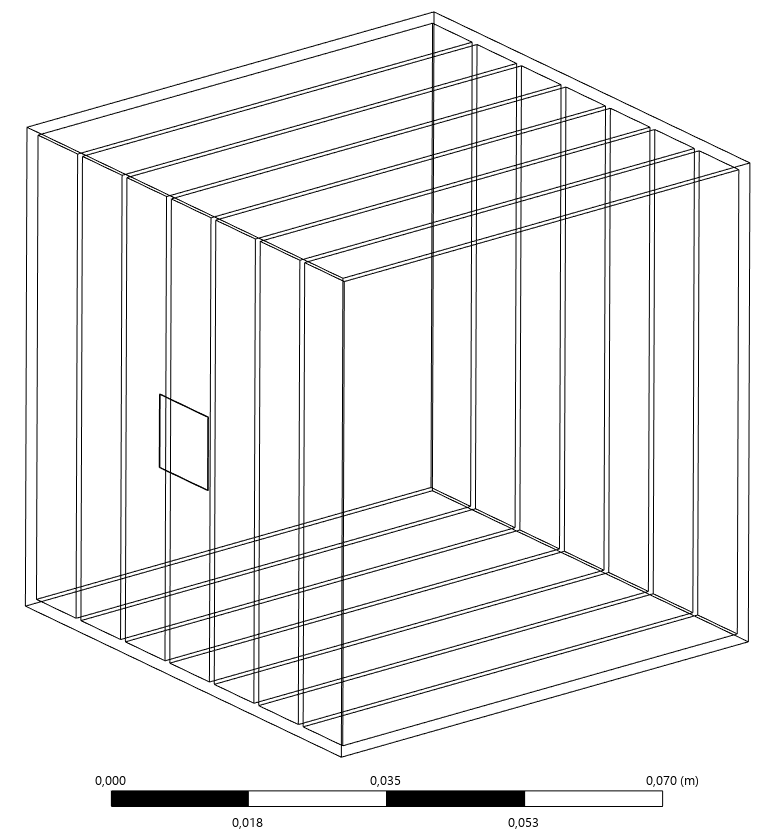
\includegraphics[height=9cm]{ansyspost/pcm/40WPCM_struktur.png}
        \caption{\ac{pcm} Struktur}\label{fig:pcm_struktur}
    \end{subfigure}
    \hfill
    \begin{subfigure}[t]{0.15\textwidth}
        \centering
        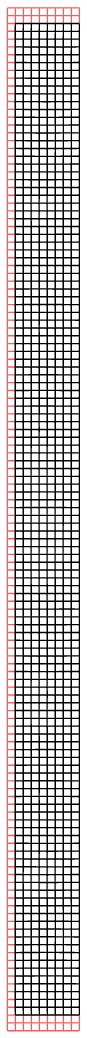
\includegraphics[height=9cm]{ansyspost/pcm/2DPCM_mesh.png}
        \caption{\ac{pcm} Mesh}\label{fig:pcm_mesh}
    \end{subfigure}
    \caption{\ac{pcm} Struktur und vereinfachtes Mesh}\label{fig:pcm_geometrien}
\end{figure}

Die Vorauslegungwurde mit folgenden Werten durchgeführt:\\
- Isotherm auf: \SI{38}{\celsius}\\
- Avionik Abwärme: \SI{40}{W}\\
- \SI{1}{m} Kontourlänge\\
- Radiator Emissionsgrad: \SI{0,91}{} (AZ-93)\\
- Radiator Absorptionsgrad: \SI{0,15}{} (AZ-93)\\
- Icosane PCM\\
- Trajektoriensimulation\\
- \SI{1}{\kilo\watt\per\meter\squared} mit 50\% dutycycle durch Rotation der Rakete\\
Zu beachten ist, dass die Radiatorleistung konstant bleibt, da das System als isotherm mit einer
infinitesimalen Temperaturerhöhung über den Schmelzpunkt hinweg angenommen wird.\\
Als nächstes sieht man die Flugdaten




\section{Aerodynamische Aufheizung}\label{sec:sim_aerodynamisch}

Speziell für die Strömungssimulationen welche keine Koppelung mit Festkörpern haben, wurde der Density-Based Solver ausgewählt und die
Simulation als 2D Steady State durchgeführt. Das Energiemodell wurde aktiviert und für das Viskositätsmodell~\cite{Irving-2021}

Die Umströmungssimulationen der Rakete wurden an \ac{maxq} orientiert, da es als Richtwert für Aerodynamische Aufheizung genommen werden kann.
Desweiteren ist der Wert unanhängig von der Vorauslegung, wodurch Ungenauigkeiten von dort getroffenen Annahmen vermieden werden.\\


als nächstes habe ich geschaut wo der maximale dynamische Druck erreicht wurde in der Vorauslegung. Die korrespondierenden Werte des Flugzustandes
habe ich dann als Boundery Conditions in der \ac{cfd}~Simulation genommen.
Um zu verifizieren, dass dort auch die maximale Aufheizung stattfindet, habe ich 1 Sekunden vorher und nachder
im Flug die BC's auch verwendet und einen Vergleich gezogen.\\
Maximaler dynamischer Druck: 112901.25708461029 Pa at 28.691 s\\
Entsprechender Flugzustand: 10244.138 m, 750.704 m/s, -51.587°C, 254.783 hPa mit entsprechender Luft Dichte \SI{0.4006}{kg/m^3}\\
Flugzustand bei 18.691 s \ac{maxq} - $\SI{10}{\second}$: 4274.387 m, 461.355 m/s, -12.784, 594.935 hPa mit entsprechender Luft Dichte \SI{0.7960}{kg/m^3}\\
Flugzustand bei 38.691 s \ac{maxq} + $\SI{10}{\second}$: 19758.652 m, 1189.968 m/s, -56.5°C, 56.93 hPa mit entsprechender Luft Dichte \SI{0.0915}{kg/m^3}\\
Flugzustand bei 48.7 s \ac{maxq} + $\SI{20}{\second}$: 32439.616 m, 1393.377 m/s, -43.269°C, 8.136 hPa mit entsprechender Luft Dichte \SI{0.01233001}{kg/m^3}\\
Da wie in~\ref{fig:spezifischer_waermestrom_maxQ_simulationen} zu sehen ist, der Zeitpunkt des maximalen dynamischen Druckes nicht im größten spezifischen
Wärmestrom resultiert, wurde mit der Simulation die den höheren spezifischen Wärmestrom ergeben hat, eine Lösungsfortsetzung durchgeführt um das Maximum zu finden.\\

\begin{figure}[H]
  \centering
  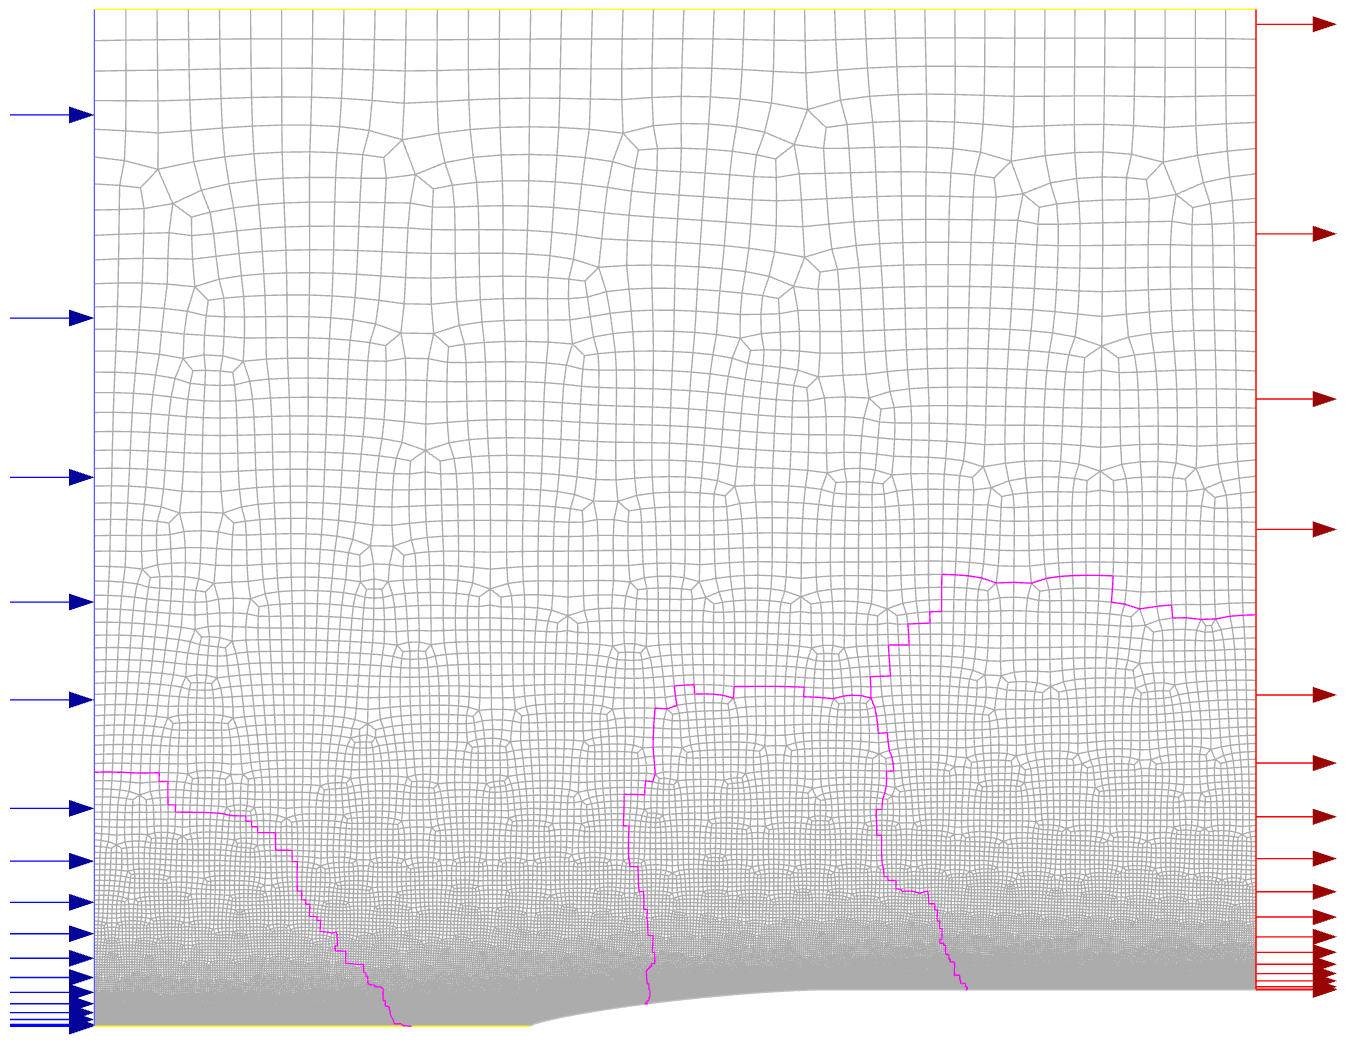
\includegraphics[width=\linewidth]{ansyspost/airflow/mesh_all.png}
  \caption{Darstellung der Außensströmungssimulation mit Meshstruktur in grau, velocity inlet in blau, pressure outlet in rot, Symmetrien in gelb und Partitionen der parallelisierung in lila}\label{fig:aussenstroemung_mesh}
\end{figure}

\begin{figure}[H]
  \centering
  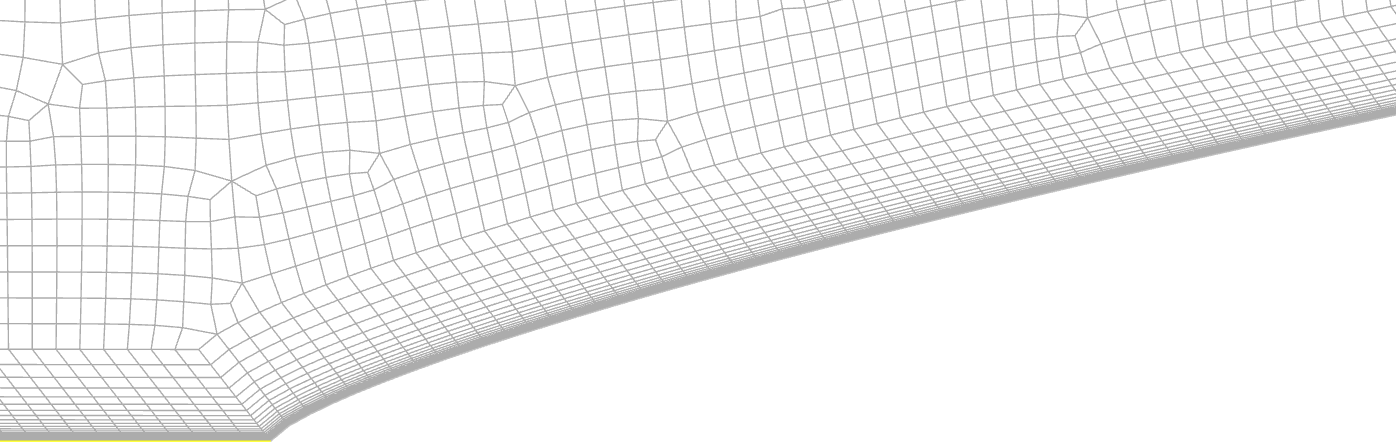
\includegraphics[width=\linewidth]{ansyspost/airflow/mesh_inflation.png}
  \caption{Schichtaufdickungen des Mesh an der Rakete}\label{fig:aussenstroemung_mesh_inflationlayers}
\end{figure}

\begin{figure}[H]
  \centering
  \includegraphics[width=\linewidth]{../../Code/maxQ_compare_heatflux.pdf}
  \caption{Spezifischer Wärmestrom an der Außenhaut bei maximalem dynamischen Druck, sowie \SI{10}{s} davor, danach und \SI{20}{s} danach}\label{fig:spezifischer_waermestrom_maxQ_simulationen}
\end{figure}

\begin{figure}[H]
  \centering
  \includegraphics[width=\linewidth]{../../Code/maxQ_compare_yplus.pdf}
  \caption{y+ Wert an der Außenhaut bei \ac{maxq}, sowie \SI{10}{s} davor, danach und \SI{20}{s} danach}\label{fig:yplus_maxQ_simulationen}
\end{figure}

\begin{figure}[H]
  \centering
  \includegraphics[width=\linewidth]{../../Code/pcm_radiator_hybrid_heatflux_with_sim.pdf}
  \caption{PCM Wärmestrom während Flug mit Simulationsergebnissen und Fit Kurve}\label{fig:pcm_waermestrom_sim}
\end{figure}

Fitted Gaussian parameters:
a=12454028.32, b=32.87, c=550.50, d=-12446646.16

\begin{figure}[H]
    \centering

    \begin{subfigure}{\textwidth}
        \centering
        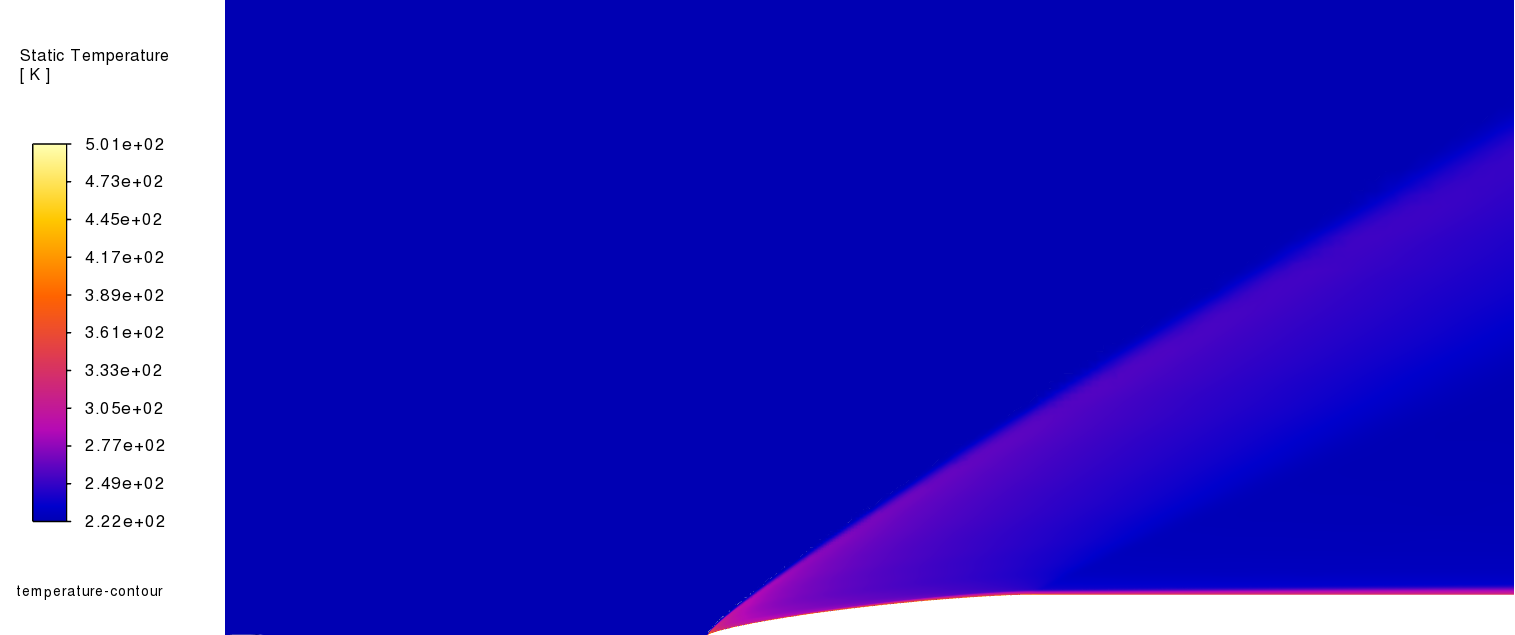
\includegraphics[height=0.23\textheight]{ansyspost/airflow/maxQ-temperature-contour.png}
        \caption{Statische Temperaturkontur der Luft}
        \label{fig:maxQ_temp_contour}
    \end{subfigure}

    \begin{subfigure}{\textwidth}
        \centering
        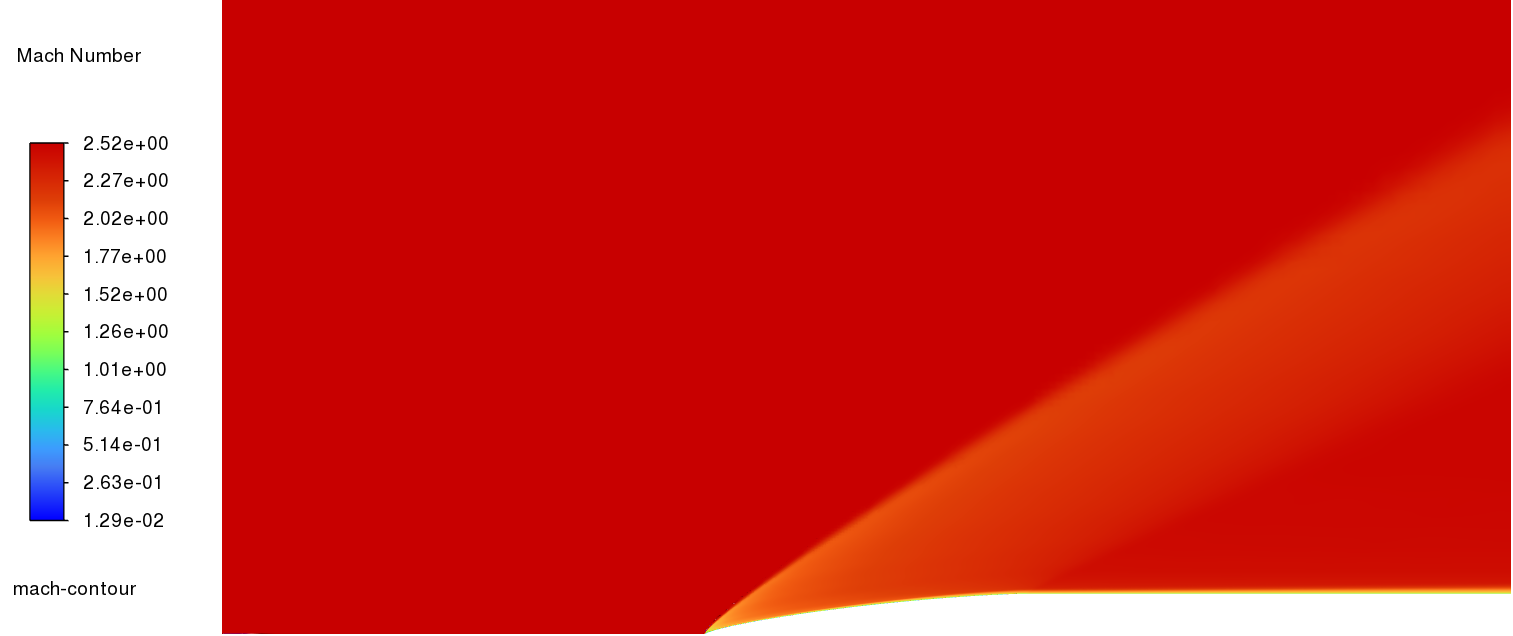
\includegraphics[height=0.23\textheight]{ansyspost/airflow/maxQ-mach-contour.png}
        \caption{Machzahlkontur der Luft}
        \label{fig:maxQ_mach_contour}
    \end{subfigure}

    \caption{\texorpdfstring{\ac{maxq}}{max Q} Konturen der Luft}
    \label{fig:maxQ_konturen}
\end{figure}

\section{PCM}\label{sec:sim_pcm}

Um in ANSYS Fluent Temperaturabhängige Stoffeigenschaften zu implementieren müssen \ac{udf} verwendet werden.
Zu der in \ref{sec:konvektion} behandelten Bossinesq-Approximation \ref{eq:bossinesque} kommen noch 

\begin{figure}[H]
  \centering
  \includegraphics[width=\linewidth]{../../Code/eicosane_cpvst_total.pdf}
  \caption{Effektive spezifische Wärmekapazität von Eicosane}\label{fig:pcm_effective_cp}
\end{figure}

\begin{figure}[H]
  \centering
  \includegraphics[width=\linewidth]{../../Code/eicosane_cpvst_sensible.pdf}
  \caption{Sensible spezifische Wärmekapazität von Eicosane}\label{fig:pcm_sensible_cp}
\end{figure}

\begin{figure}[H]
  \centering
  \includegraphics[width=\linewidth]{../../Code/approximate_acceleration_over_time.pdf}
  \caption{Approximiertes Beschleunigungsprofil}\label{fig:approximierte_beschleunigung}
\end{figure}

\ref{fig:approximierte_beschleunigung} zeigt das Beschleunigungsprofil, welches in der Simulation verwendet wurde. Zu beachten
ist, dass Beschleunigungsspitzen durch den Fallschirm, wie sie in~\ref{fig:acceleration_over_time} gesehen
werden können, ignoriert werden, da diese in einer Überschätzung der Beschleunigung und der Konvektionsvorgänge resultieren würden.


\begin{figure}[H]
    \centering

    % Left figure
    \begin{minipage}[t]{0.485\textwidth}
        \centering
        \setlength{\tabcolsep}{1pt} % reduce subfigure spacing
        % Legend vertically centered & with extra space to right
        \begin{subfigure}[t]{0.16\textwidth}
            \centering
            \raisebox{0.7\height}{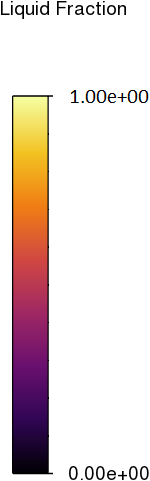
\includegraphics[height=0.2\textheight]{ansyspost/pcm/liquid-fraction-legend.png}}
        \end{subfigure}%
        \hspace{2mm}% extra space between legend and first image
        \begin{subfigure}[t]{0.2\textwidth}
            \centering
            
\includegraphics[height=0.5\textheight]{ansyspost/pcm/liquid-fraction-300.png}
            \caption{\SI{300}{\second}}\label{fig:liquid_fraction_300}
        \end{subfigure}%
        \begin{subfigure}[t]{0.2\textwidth}
            \centering
            
\includegraphics[height=0.5\textheight]{ansyspost/pcm/liquid-fraction-600.png}
            \caption{\SI{600}{\second}}\label{fig:liquid_fraction_600}
        \end{subfigure}%
        \begin{subfigure}[t]{0.2\textwidth}
            \centering
            
\includegraphics[height=0.5\textheight]{ansyspost/pcm/liquid-fraction-900.png}
            \caption{\SI{900}{\second}}\label{fig:liquid_fraction_900}
        \end{subfigure}%
        \begin{subfigure}[t]{0.2\textwidth}
            \centering
            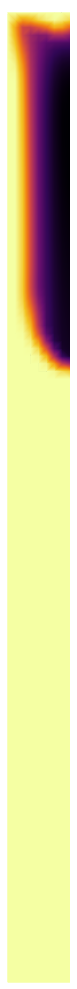
\includegraphics[height=0.5\textheight]{ansyspost/pcm/liquid-fraction-1200.png}
            \caption{\SI{1200}{\second}}\label{fig:liquid_fraction_1200}
        \end{subfigure}
        \caption{Flüssigkeitsanteil Konturen. Die Legende bezieht sich auf~\ref{fig:liquid_fraction_1200}}
        \label{fig:liquid_frac_kontur}
    \end{minipage}
    \hspace{2mm} % small horizontal space
    % Right figure
    \begin{minipage}[t]{0.485\textwidth}
        \centering
        \begin{subfigure}[t]{0.16\textwidth}
            \centering
            \raisebox{0.7\height}{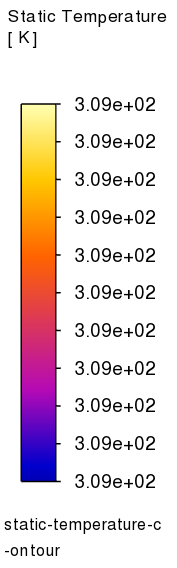
\includegraphics[height=0.2\textheight]{ansyspost/pcm/temperature-legend.png}}
        \end{subfigure}%
        \hspace{2mm}% extra space between legend and first image
        \begin{subfigure}[t]{0.2\textwidth}
            \centering
            
\includegraphics[height=0.5\textheight]{ansyspost/pcm/static-temperature-300.png}
            \caption{\SI{300}{\second}}\label{fig:temperatur_300}
        \end{subfigure}%
        \begin{subfigure}[t]{0.2\textwidth}
            \centering
            
\includegraphics[height=0.5\textheight]{ansyspost/pcm/static-temperature-600.png}
            \caption{\SI{600}{\second}}\label{fig:temperatur_600}
        \end{subfigure}%
        \begin{subfigure}[t]{0.2\textwidth}
            \centering
            
\includegraphics[height=0.5\textheight]{ansyspost/pcm/static-temperature-900.png}
            \caption{\SI{900}{\second}}\label{fig:temperatur_900}
        \end{subfigure}%
        \begin{subfigure}[t]{0.2\textwidth}
            \centering
            
\includegraphics[height=0.5\textheight]{ansyspost/pcm/static-temperature-1200.png}
            \caption{\SI{1200}{\second}}\label{fig:temperatur_1200}
        \end{subfigure}
        \caption{Konturen der statischen Temperatur. Die Legende bezieht sich auf~\ref{fig:temperatur_1200}}
        \label{fig:static_temperature_kontur}
    \end{minipage}

\end{figure}


\begin{lstlisting}[language=C, float, caption={Boussinesq-Approximation des Auftriebs im \ac{pcm} in der \ac{udf} eicosane.c}, label={lst:udf_bossinesque}]
//Y-momentum source
DEFINE_SOURCE(Boussinesq_momentum_source,cell,thread,dS,eqn)
{
	double Temp, source, acc;
	Temp=C_T(cell,thread);

	double t = CURRENT_TIME;

	if (t < 20)
		acc = 34.81;
	else if (t < 50)
		acc = 109.81;
	else if (t < 150)
		acc = 19.62;
	else
		acc = 9.81;

	source=-Rol_pcm*acc*TEC*(Temp-Tr);  //negative for -Y down
	dS[eqn]=-Rol_pcm*acc*TEC; 			//negative for -Y down
	return source;
}
\end{lstlisting}

\begin{figure}[H]
  \centering
  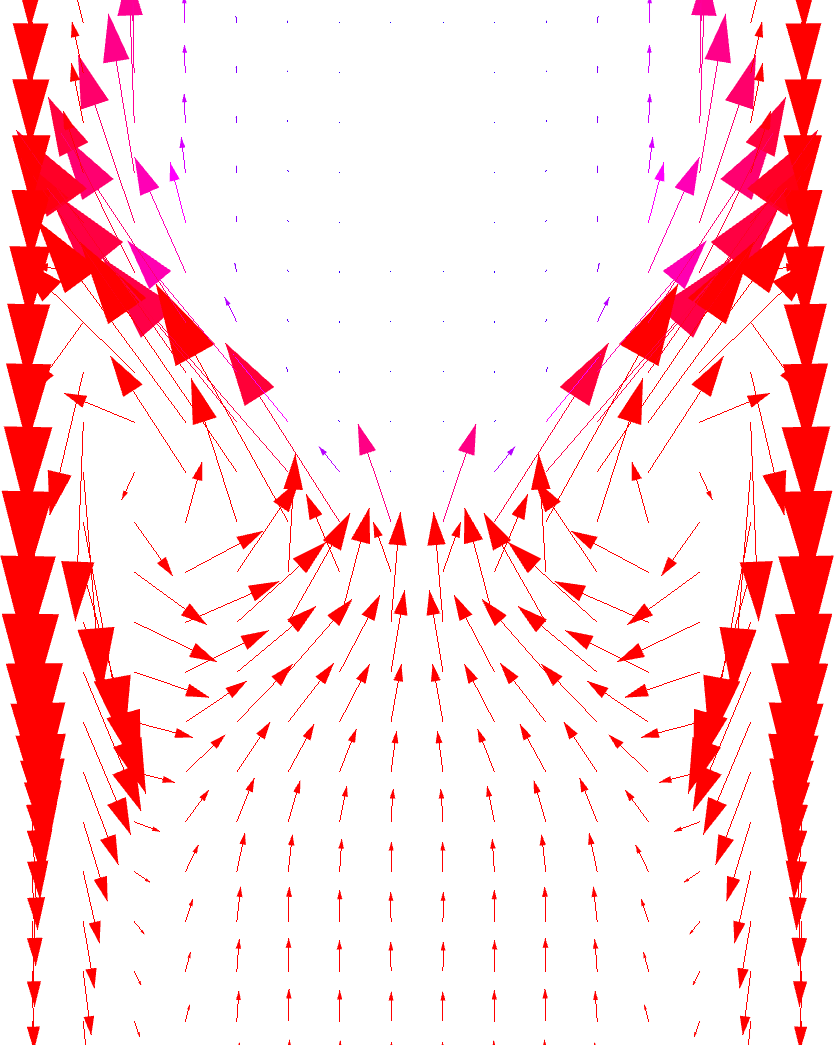
\includegraphics[height=0.4\textheight]{ansyspost/pcm/velocity-vector-close-stitched-900.png}
  \caption{Geschwindigkeitsvektoren der Konvektionswirbel einer, durch Nachbearbeitung, vervollständigten Zelle
  bei \SI{900}{\second}. Darstellung der weiteren Zeitschritte ist in~\ref{fig:pcm_static_temperature_kontur} zu finden.}\label{fig:pcm_vectoren_stitched}
\end{figure}